\documentclass[11pt, a4paper]{article}
\title{Wacky Racers 2024 Instructions}
\author{Michael Hayes}
\date{Version 1.110, \today}

\usepackage[margin=1in]{geometry}
\usepackage{parskip}
\usepackage{float}
\usepackage{todonotes}
\presetkeys{todonotes}{inline}{}
\usepackage{graphicx}
\usepackage[T1]{fontenc}
\usepackage{makecell}
\usepackage[breaklinks=true]{hyperref}
\usepackage{tabularx}
\usepackage{subcaption}
\usepackage{listings}
\usepackage{siunitx}
\usepackage{circuitikz}
\usepackage{tikz}
\usetikzlibrary{arrows}

\newcommand{\code}[1]{\texttt{#1}}

\newcommand{\fredyemail}{\url{mailto:fredy.youssif@canterbury.ac.nz}}
\newcommand{\scottemail}{\url{mailto:scott.lloyd@.canterbury.ac.nz}}
\newcommand{\diegoemail}{\url{mailto:diego.ramirez@canterbury.ac.nz}}

\newcommand{\fredy}{\href{mailto:fredy.youssif@pg.canterbury.ac.nz}{Fredy Youssif}}
\newcommand{\scott}{\href{mailto:scott.lloyd@.canterbury.ac.nz}{Scott Lloyd}}
\newcommand{\diego}{\href{mailto:diego.ramirez@canterbury.ac.nz}{Diego Ramirez}}

\newcommand{\theguide}{\href{https://eng-git.canterbury.ac.nz/wacky-racers/wacky-racers/-/blob/master/doc/guide/guide.pdf}{The Wacky Racers Guide}}


\begin{document}
\maketitle

\section{Introduction}

The purpose of this assignment is to design, build, and program an
embedded system using an ARM microcontroller and surface mount
technology.

The goal for each group of four students is to build a remote
controlled vehicle (the Wacky Racer) and its controller (the Wacky
Hat).  At the conclusion of the assignment there will be a dastardly race!

Each group is comprised of two sub-groups of two students.  One of
these subgroups constructs the Wacky Racer and the other constructs
the Wacky Hat.  You may be asking why is the Wacky Hat called the
Wacky Hat?  Well, a hat that controls a remote vehicle using head
motions is not an ordinary hat!


\section{Requirements}

The following requirements are mandatory if you wish to maximise your
marks.


\subsection{Wacky racer}

\begin{enumerate}
\item The chassis is to be constructed by each group.  These can be 3-D printed,
  constructed from Perspex or wood, etc.  A standard chassis is available from
  the Electronics Lab technician (Diego Ramirez).  The electronics must be
  visible on top of the chassis.
\item Have a standard working bump sensor (supplied).
\item Locomotion can only use two 6\,V DC motors (supplied).
\item Everything must be powered from a single 5-cell NiMH battery pack (supplied).
\item Use a single four layer printed circuit board of dimension 85\,mm$\times$64\,mm.
\item Use an ARM microcontroller (Atmel SAM4S).
\item Drive the motors using H-bridges (Texas Instruments DRV8833 dual
  H-bridge).
\item Regulate the nominal battery voltage to 5\,V with a buck
  regulator IC (ADP2302ARDZ-50).
\item Be decorated with an LED tape (supplied) controlled by the MCU.
\item Use a USB interface for debugging.
\item Use a serial wire debug interface for MCU programming/debugging.
\item Have adequate battery fusing and reverse polarity protection.
\item Have a pushbutton connected to the MCU to enter and wake from
  low-power mode (optional).
\item Have a red LED to indicate errors.
\item Have a green LED to indicate status.
\item If the battery voltage drops below 5\,V, the red LED should flash and high power draw devices should be disabled.
\item Interface to the Wacky Hat with a Nordic nRF24 SMD radio module
.
%\item Have a mounted RFID card (supplied) that can be read by the Wacky ramps.
\item Be humorous.
\end{enumerate}

\hspace{120mm}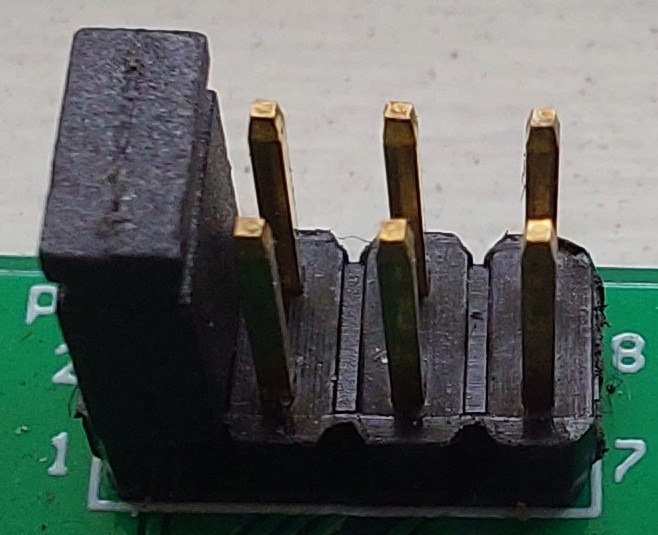
\includegraphics[width=3cm]{../guide/figs/jumpers4.jpg}


Each Wacky Racer can have a dastardly means of hindering another
team's Wacky Racer.  However, you cannot:
%
\begin{itemize}
\item Damage or destroy another Wacky racer (except in the battle royale)
\item Damage the venue
\item Injure a spectator
\item Jam the radio signals
\end{itemize}


\vspace{1cm}

\begin{figure}[h]
    \centering
    \input{racer_top_level.tex}
    \caption{Racer board top level diagram.}
\end{figure}


\vfill\pagebreak

\subsection{Wacky hat}


\begin{enumerate}
\item Construct a Wacky Hat that contains all the electronics.
\item Everything must be powered from a single 5-cell NiMH battery pack (supplied).
\item Have adequate battery fusing and reverse polarity protection.
\item Use a single four layer printed circuit board of dimension 85\,mm$\times$64\,mm.
\item Use an ARM microcontroller (Atmel SAM4S).
\item Regulate the nominal 6\,V battery voltage to 5\,V with a buck
  regulator IC (ADP2302ARDZ-50).
\item Be decorated with an LED tape (supplied) controlled by the MCU.
\item Use an I2C accelerometer (ADXL345) for head motion detection.
\item Use a USB interface for debugging.
\item Use a serial wire debug interface for MCU programming/debugging.
\item Have a pushbutton connected to the MCU to enter and wake from
  low-power mode (optional).
\item If the battery voltage drops below 5\,V, the red LED should flash and high power draw devices should be disabled.
\item Have an active-high red LED to indicate errors.
\item Have an active-high green LED to indicate status.
\item Play sound when the bumper is hit.
\item Interface to the Wacky Racer with a Nordic nRF24 SMD radio module.
\item Have jumpers or switches to select four radio channels.
\item Be humorous.
\end{enumerate}

%\vspace{1cm}

\begin{figure}[h]
  \centering
  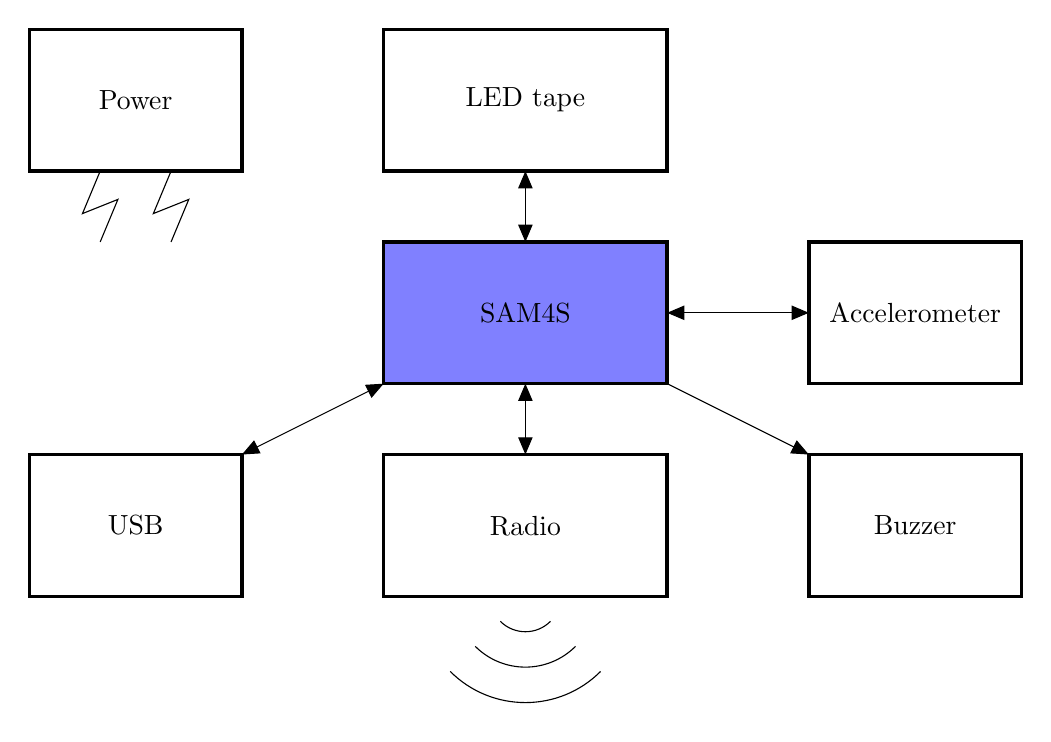
\begin{tikzpicture}[scale=0.9]

  \draw[black, very thick, fill=blue!50] (-2, -1) rectangle (2, 1);
    \node at (0, 0) {SAM4S};

    % Accelerometer
    \draw[black, very thick] (4, -1) rectangle (7, 1);
    \node at (5.5, 0) {Accelerometer};
    \draw[triangle 45-triangle 45] (2, 0) -- (4, 0);

    % Buzzer
    \draw[black, very thick] (4, -2) rectangle (7, -4);
    \node at (5.5, -3) {Buzzer};
    \draw[-triangle 45] (2, -1) -- (4, -2);

    % LED tape
    \draw[black, very thick] (-2, 2) rectangle (2, 4);
    \node at (0, 3) {LED tape};
    \draw[triangle 45-triangle 45] (0, 1) -- (0, 2);

    % Radio
    \draw[black, very thick] (-2, -2) rectangle (2, -4);
    \node at (0, -3) {Radio};
    \draw[triangle 45-triangle 45] (0, -1) -- (0, -2);
    \draw (0.354, -4.354) arc (-45:-135:0.5);
    \draw (0.707, -4.707) arc (-45:-135:1);
    \draw (1.061, -5.061) arc (-45:-135:1.5);

    % Power
    \draw[black, very thick] (-4, 2) rectangle (-7, 4);
    \node at (-5.5, 3) {Power};
    \draw (-5, 2) -- (-5.25, 1.4) -- (-4.75, 1.6) -- (-5, 1);
    \draw (-6, 2) -- (-6.25, 1.4) -- (-5.75, 1.6) -- (-6, 1);

    % USB
    \draw[black, very thick] (-4, -2) rectangle (-7, -4);
    \node at (-5.5, -3) {USB};
    \draw[triangle 45-triangle 45] (-2, -1) -- (-4, -2);


\end{tikzpicture}

  \caption{Racer hat top level diagram.}
\end{figure}


\vfill\pagebreak

\section{Assignment schedule}

The planned activities for the timetabled labs in the Embedded Systems
Lab (ESL) are:
%
\begin{flushleft}
  \begin{tabular}{ c l l }
    Week            &  Assistance  &  Assessment \\
    \hline \hline
    T1-1 & Altium tutorial 1 (schematics)  & \\
    T1-2 & Altium help      & \\
    T1-3 & Schematic review & Schematic submission for review (Monday 9am) \\
    T1-4 & Altium tutorial 2 (PCB) &          \\
    T1-5 & Altium help      & PCB submission 1    \\
    T1-6 & Altium help      & PCB submission 2    \\
    \hline
    B-1  & (break)          &                   \\
    B-2  & (break)          &                   \\
    B-3  & (break)          &                   \\
    \hline
    T2-1 & General          &                   \\
    T2-2 & General          & Blinky            \\
    T2-3 & General          & Accelerometer/motors        \\
    T2-4 & General          & Radio control     \\
    T2-5 & General          & Functionality     \\
    T2-6 & Competition      & Competition, critique  \\
  \end{tabular}
\end{flushleft}


Notes:
%
\begin{enumerate}
\item There are two lab streams.  Your group will need to sign up to
  one of the streams.  Choose an odd numbered group for the Wednesday
  1--3 pm stream or an even numbered group for the Wednesday 3--5 pm
  stream.

\item There may be a 6--10 day delay for the PCBs to be manufactured
  from the time of submission.  You will then need to book an assembly
  session in the SMT lab provided you have done the SMT lab induction.

\item Do not underestimate the blinky milestone.  The program is
  trivial; you just have to flash an LED.  However, it requires having
  a functional PCB, a functional toolchain, and the ability to
  download code into the microcontroller's flash memory.

\end{enumerate}


\section{Assessment}

The marks breakdown (max. 0x64) is:
%
\begin{flushleft}
  \begin{tabular}{ll}
    PCB submission & 0--0xa marks\\
    Blinky milestone  & 0x5 marks\\
    Accelerometer/motor milestone  & 0x5 marks\\
    Radio control milestone  & 0x5 marks\\
    Functional assessment & 0--0x14 marks \\
    Board inspection & 0--0x1e marks \\
    Competition & 0--0xa marks \\
    Individual critique & 0--0xf marks \\
  \end{tabular}

\end{flushleft}

\subsection{Milestones}

There are five milestones.  To achieve the associated marks, they must
be demonstrated to a T.A. by the end of the lab for your allotted
stream.  If you need an exception to this, see \fredy\ with a
\emph{very} good reason such as isolating with COVID.  The milestone
requirements are:
%
\begin{description}
\item [Schematic review] Submit your A3 schematic on Learn for
  review.  Lose 10 marks if you miss the submission time.

\item [PCB submission] Submit your PCB design to Learn for
  manufacture.  To encourage early submission there is a sliding scale
  for marks depending on when the PCB is submitted, see table.  After
  week 6, there is a 10 mark penalty per week.  \textbf{NB, a rushed
    PCB design will cause you more grief, more PCB rework, and a lower
    mark for the inspection.}

  It is not possible for me to cover all aspects of PCB design before
  your PCB submission.  I recommend you read the lecture notes for
  power supply decoupling and crosstalk.

  \begin{tabular}{llll}
    Week & Submission day & Cut-off time  & Mark \\ \hline
    5    & Monday       & 1.00 pm & 10 \\
    5    & Tuesday      & 1.00 pm & 9 \\
    5    & Wednesday    & 1.00 pm & 8 \\
    5    & Thursday     & 1.00 pm & 7 \\
    5    & Friday       & 1.00 pm & 6 \\
    6    & Monday       & 1.00 pm & 5 \\
    6    & Tuesday      & 1.00 pm & 4 \\
    6    & Wednesday    & 1.00 pm & 3 \\
    6    & Thursday     & 1.00 pm & 2 \\
    6    & Friday       & 1.00 pm & 1  \\
  \end{tabular}

\item [Blinky] Demonstrate that can blink an LED controlled by the SAM4S.

\item [Accelerometer/motors] For the Wacky Hat, demonstrate output of
  accelerometer readings to a PC using USB CDC and generate a PWM
  signal with a frequency proportional to the tilt angle of the
  accelerometer.

  For the Wacky Racer, demonstrate generation of a PWM signal with a
  duty set from a terminal program using USB CDC.

\item[Radio control]

  Demonstrate sending commands from the Wacky Hat to the Wacky Racer
  and vice-versa over a radio link.

%  Demonstrate sending commands from the Wacky Hat to the Wacky Racer
%  over a radio link.
\end{description}

\textbf{If you cannot show the functionality of a previous milestone
  during any assessment, you will fail that assessment and loose any
  marks from the previous milestone.}


\subsection{Functionality assessment}

Functionality requirements:
%
\begin{flushleft}
  \begin{tabular}{l|l}
    Wacky racer & Wacky hat \\ \hline \hline
    Blink LED                      & Blink LED \\
    Drives LED tape                & Drives LED tape \\
    Drive motors forward/backward  & Read from accelerometer \\
    Speed control of motors        & Calculate speeds from accelerometer \\
    Steering control               & Joystick control \\
    Receive/send radio message     & Receive/send radio message \\
    Jumper selectable radio channel & Jumper selectable radio channel  \\
    Dies on bump                   & Plays sound on bump \\
    Low voltage indication         & Low voltage indication \\
  \end{tabular}
\end{flushleft}
%
Marks are allocated on how well things work.  Up to 5 bonus marks can
be awarded for extra functionality such as:
%
\begin{flushleft}
  \begin{tabular}{l|l}
    Wacky racer                & Wacky hat \\ \hline \hline
    Dastardly stuff            & Plays interesting sounds \\
    Sleep mode                 & Sleep mode \\
  \end{tabular}
\end{flushleft}

Sleep mode is where you shutdown the MCU to save energy and use a
pushbutton to awake the MCU via an interrupt.  Is is easy to get wrong
and hard to save every microamp.

\subsection{Competition}

The competition is a race around an obstacle course.  Marks will be
awarded every time you pass over a Wacky Ramp in the correct order.

%These ramps have an RFID card reader that will detect your Racer if
%you have correctly fitted an RFID card.  The Wacky Ramps change colour
%when they detect a Wacky Racer.

To be awarded any marks for the race:
%
\begin{enumerate}
\item Your vehicle must stop for at least 5\,s if the bumper is hit.

\item Your vehicle must be controlled by motions of the Wacky hat
  sitting on someone's head.
\end{enumerate}

After the races, there will be a battle royale where the last
operational wacky racer wins.  Hitting the bumper of an opponents
wacky racer removes them from the battle.

Marks will also be awarded for wackiness, group costumes, etc.




\subsection{PCB inspection}

This is assessed after the competition.  The categories are:
%
\begin{enumerate}
\item Layout (component placement etc.)
\item Construction (tidiness, rework, etc.)
\item Testability
\item Power supplies (routing, decoupling, etc.)
\end{enumerate}


\vfill\pagebreak
\section{Schedule}

\begin{description}
\item [Week~1]\mbox{}\\[-0.4cm]

  \begin{itemize}
  \item Form a group of four and register your group on Learn.  If you
    cannot form a group of 4, contact \fredy.

  \item Read the Requirements section in this document.

  \item Read the System Design section in the \theguide.

  \item Attempt Altium schematic tutorial.

  \end{itemize}

\item [Week~2]\mbox{}\\[-0.4cm]

  \begin{itemize}
  \item Peruse the datasheets of the key components.

  \item Start your schematic design.

  \end{itemize}

\item [Week~3]\mbox{}\\[-0.4cm]

  \begin{itemize}

    %  \item Sign-up for a SMT lab induction
  \item Submit your Altium schematic for review.

  \item Watch review feedback session.

  \item Correct your schematic.

  \end{itemize}

\item [Week~4]\mbox{}\\[-0.4cm]

  \begin{itemize}
  \item Attempt Altium PCB tutorial.

  \item Start your PCB layout.
  \end{itemize}

\item [Week~5]\mbox{}\\[-0.4cm]

  \begin{itemize}
  \item Watch SMT lab induction video.

  \item Submit PCB design (early round).
  \end{itemize}

\item [Week~6]\mbox{}\\[-0.4cm]

  \begin{itemize}
  \item Submit PCB design (late round).
  \end{itemize}

%\item [Week~7]\mbox{}\\[-0.4cm]


%\item [Week~8]\mbox{}\\[-0.4cm]


\item [Week~9]\mbox{}\\[-0.4cm]

  \begin{itemize}
  \item Populate and test PCB.
  \end{itemize}


\item [Week~10]\mbox{}\\[-0.4cm]

  \begin{itemize}
  \item Populate and test PCB.
  \item Demonstrate blinky program.
  \end{itemize}

\item [Week~11]\mbox{}\\[-0.4cm]

  \begin{itemize}
  \item Demonstrate blinky program.
  \end{itemize}

\item [Week~12]\mbox{}\\[-0.4cm]

  \begin{itemize}
  \item Demonstrate accelerometer/motors functionality.
  \end{itemize}

\item [Week~13]\mbox{}\\[-0.4cm]

  \begin{itemize}
  \item Demonstrate radio control.

  \item Plan your costumes!
  \end{itemize}

\item [Week~14]\mbox{}\\[-0.4cm]

  \begin{itemize}
  \item Demonstrate full functionality.

  \item Prepare your costumes and dastardly stuff!
  \end{itemize}

\item [Week~15]\mbox{}\\[-0.4cm]

  \begin{itemize}
  \item Practice control of your wacky racer.
  \item Attend wacky race.
  \item Submit PCB for inspection (box in SMT lab).
  \item Return chassis, batteries, and ST-link programmers.
  \item Submit individual critique to Learn.
  \end{itemize}

\end{description}



\section{Technical stuff}

Read this section carefully.  There are clues as to how we mark your PCBs.

\subsection{Version control}

Use version control for everything, or else!  Learning git is
frustrating but is a skill you will not regret, see \theguide\ for
details.

Your group leader should create a forked copy of the wacky-racers git project
and then add the other group members to the project.  This can be done by:

\begin{enumerate}
\item Go to \url{https://eng-git.canterbury.ac.nz/wacky-racers/wacky-racers}

\item Click `Fork' button.  This will create a copy of the main repository for the project.

\item Click on the `Settings' menu then click the `Expand' button for
`Sharing and permissions'.  Change `Project Visibility' to `Private'.

\item Click on the `Members' menu and add group members as Developers.

\item Using a bash terminal (or other useful shell), enter the command:

\lstset{language=bash}
\lstset{basicstyle=\ttfamily\small}
\lstset{keywordstyle=\color{black}\ttfamily}
\lstset{breaklines}

\begin{lstlisting}
  $ git clone https://eng-git.canterbury.ac.nz/your-userid/wacky-racers.git
\end{lstlisting}

If you do not want to have to enter your password for every git
push/pull operation, you should set up ssh-keys and use the git URL instead:

\begin{lstlisting}[breaklines]
  $ git clone git@eng-git.canterbury.ac.nz:your-userid/wacky-racers.git
\end{lstlisting}

\item Add a remote URL for the main repository.
%
\begin{lstlisting}[breaklines]
  $ cd wacky-racers
  $ git remote add upstream https://eng-git.canterbury.ac.nz/wacky-racers/wacky-racers.git
\end{lstlisting}
%
Again if you do not want to manually enter your password, you can use:
%
\begin{lstlisting}[breaklines]
  $ cd wacky-racers
  $ git remote add upstream git@eng-git.canterbury.ac.nz:wacky-racers/wacky-racers.git
\end{lstlisting}

\item If we add more demo code or tweak the instructions in the main
repository, you can get the updated stuff using:
%
\begin{lstlisting}[breaklines]
  $ git pull upstream master
\end{lstlisting}
\end{enumerate}


\subsection{Schematics}

\begin{enumerate}
\item Attempt the Altium tutorial on Learn.

\item Read the \theguide.

\item Add your name, your partner's name, and your group number to the
  title block.

\item Save PDF files of your schematics in your source repository.
  \textbf{Note, when debugging your PCBs, we will not help you until
    you show us your printed A3 schematic}.

\item I bet that you will not have enough test points to clip an
  oscilloscope probe to.  Do not think you can hold the probe tip
  against an MCU pin without shorting something.  Ensure you give a
  meaningful name to the test point in its comment field.

  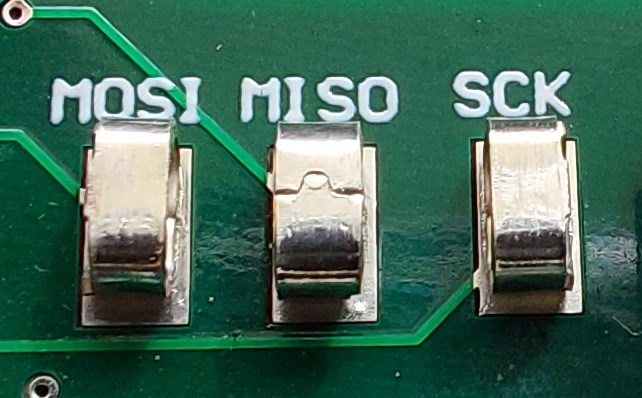
\includegraphics[width=5cm]{../guide/figs/testpoints.jpg}  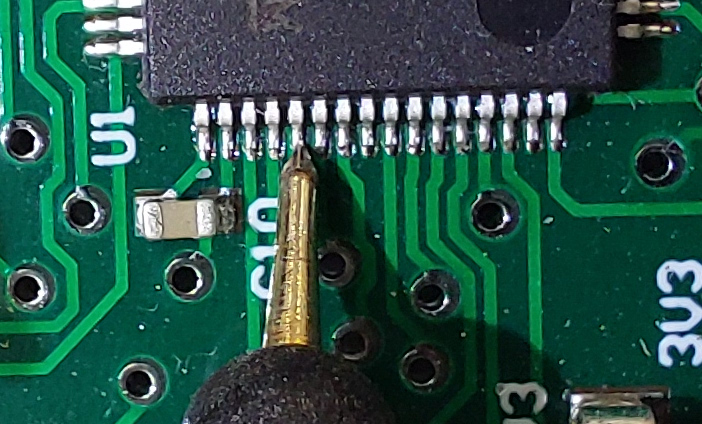
\includegraphics[width=5cm]{../guide/figs/micro_probe_zoom.jpg}

\item Ground test points are essential for an oscilloscope earth clip.
  A U-shaped piece of wire soldered between two holes is good for this.
  Keep ground test points clear of other test points since the earth
  clip may short between them.  You will probably require at least two
  ground points on opposite sides of the PCB.

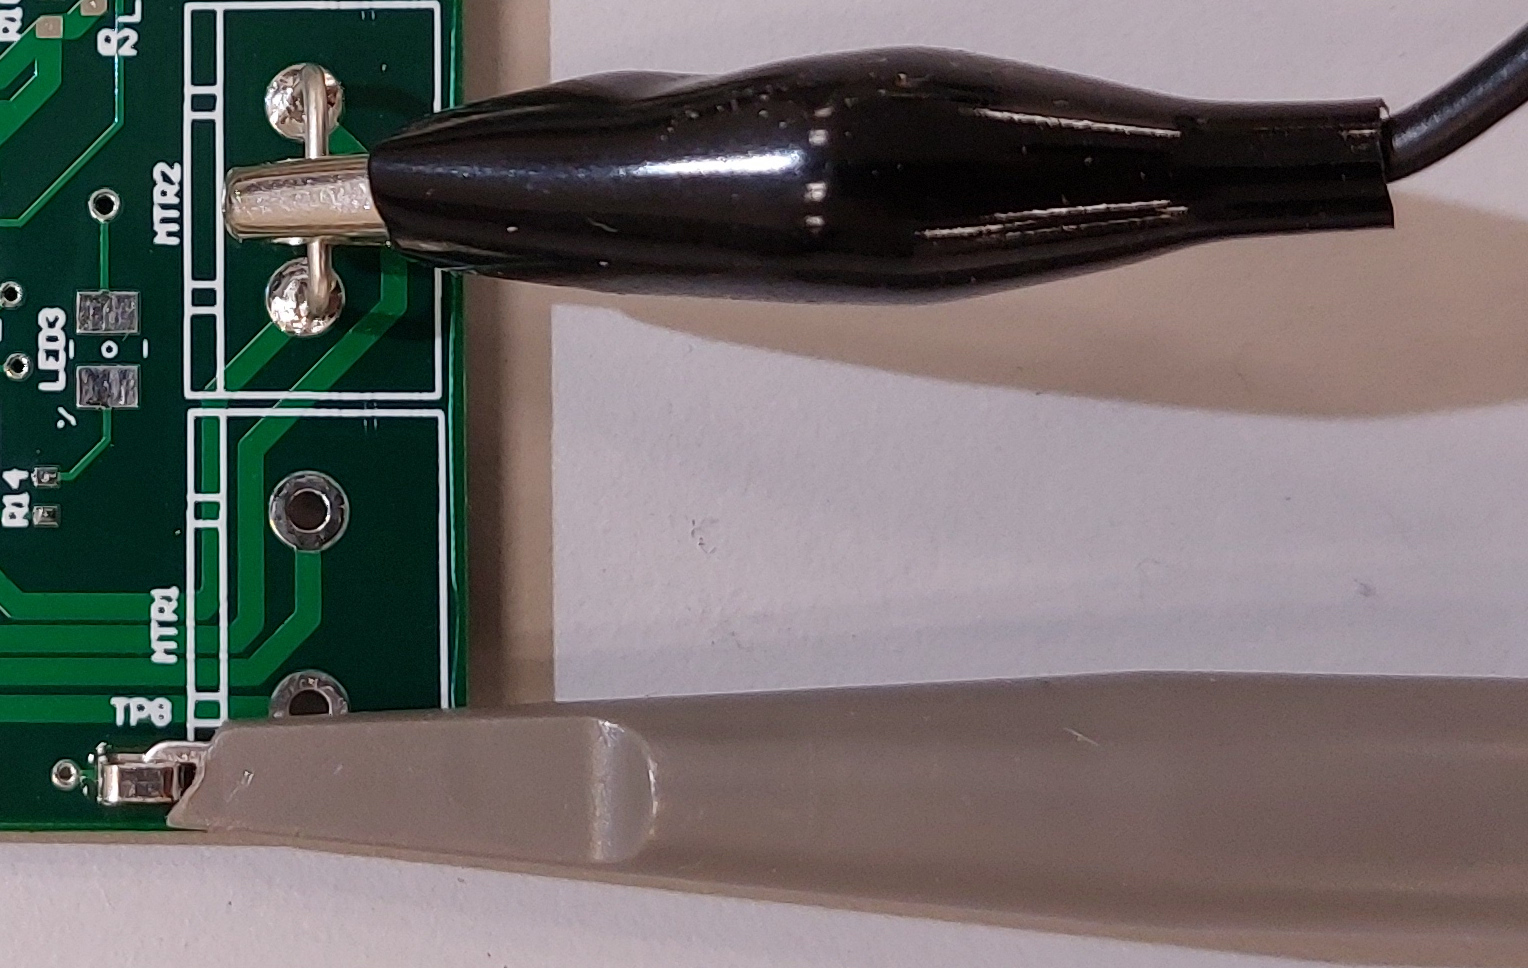
\includegraphics[width=5cm]{../guide/figs/scope_probe_testpoints.jpg}

\item Checking the schematic is the most crucial part of the
  assignment.  If the schematic is wrong then your PCB will be wrong
  and you will need to do rework.  So, schematics must be thoroughly
  checked by another person.

\item It would be useful to have jumpers connected to PIO pins so
  that you can configure your board.

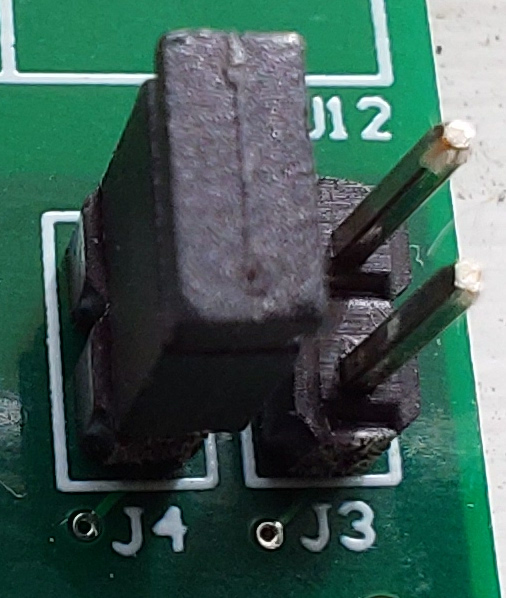
\includegraphics[width=2cm]{../guide/figs/jumpers.jpg}

\item In case you forget something, I suggest running some spare PIO
  pins from the MCU to some pads or a connector.

\end{enumerate}


\subsection{PCBs}

\begin{enumerate}
\item Your four-layer PCBs are going to be manufactured in batches.
  There is at least a week turnaround time to get the boards made.

\item It is important that you check footprints for parts they you
  create.  We will impose a 10\% penalty for each rerun of a PCB, say
  due to a footprint mistake.  Get your partner to check.

\item In Altium, turn off the test point designators and turn on
  comments instead. This lets you give them human readable names to
  make your lives easier.

\item PCB layouts must be thoroughly checked by another person.

\item A PCB track can blow faster than a fuse. So keep high current
  tracks fat and short.

\item Clearly mark the positive and negative battery connections on
  the silk screen.

\item Some of the chips can get hot so thermal considerations are
  required.  Follow the manufacturers' guidelines in the datasheets.

\item The switching regulators can interfere with the radios.

\item Use a design rule check to see if any of the following
  constraints are violated:
%
\begin{itemize}
\item Minimum trace width (0.15\,mm)
\item Minimum trace clearance (0.15\,mm)
\item Minimum via size (0.3\,mm hole, 0.6\,mm outer diameter)
\item Minimum hole size (0.3\,mm)
\item Minimum annular ring (0.1\,mm)
\end{itemize}
%
For every violation of one these rules, we will deduct 1\% from your
final mark.

\item Check the checklist in the \theguide\ before submission.
\end{enumerate}


\subsection{Assembly}

\begin{enumerate}
\item Finding shorts is extremely frustrating so maximise clearances
  and test for shorts before populating components.

\item Components can be put through the oven on the reverse side
  although heavy components may need to be glued.

\item Never assume where pin 1 is on an IC; check the datasheet.
  5--10\% of groups will get this wrong.

\end{enumerate}


\subsection{Software}

\begin{enumerate}
\item Read the \theguide.

\item If you are not using version control, you are foolish.

\item Inspect the sample code in the \code{test-apps} directory.

\item If you are trying to program the SAM4S for the first time and
  are feeling tired or impatient, then do something else.
\end{enumerate}


\subsection{Debugging}

\begin{enumerate}
\item Start running small programs (such as the provided demo
  programs) to test each feature separately.

\item An oscilloscope is your friend.  Use normal mode for digital
  signals.

\item It is possible to use the GDB debugger but you need to know what
  you are doing, especially with optimised code (ask the TAs).

\item Drawing a diagram of what you think is happening is highly
  recommended. A simple circuit diagram or timing diagram will often
  help you realise what you have missed and let you fix it without
  asking for help.

\end{enumerate}


\subsection{Possibly asked questions with answers}

\begin{itemize}
\item \emph{Why use the SAM4s MCU?}  For this application most MCUs
  would suffice, even an 8-bit AVR microcontroller.  To level the
  playing field, I have chosen a MCU most students would not have used
  before.  This is an ARM based MCU made by Atmel I have used this in
  a number of projects.  Indeed we used to teach this chip in ENCE361.
  There are many other similar MCUs made by different manufacturers
  such as the STM32 that would just as suitable.

\item \emph{Why use a four layer PCB?}  Come to lectures to find out!

\item \emph{Why use 7.2\,V NiMH batteries for the Wacky Racers?}
  These were a legacy of previous Wacky Racers.  They are also safer
  than lithium batteries with sleep-deprived students.

%% \item \emph{Why can't I program my device using Windows?} Due to
%%   various aspects of the Windows ecosystem, setting up a fully
%%   functional build environment is more complicated, will often vary
%%   from machine to machine, will often break filepaths, and will often
%%   cause bizarre compilation errors. Use at your own risk, we will not
%%   assist in debugging issues related to Windows.

\end{itemize}


\section{Assistance}

\fredy\ is our senior tutor for embedded systems and is in charge of
the assignment.  He is supported by a team of TAs and technicians
\scott\ (\scottemail) and \diego\ (\diegoemail).  \scott\ has his
office in the Surface Mount Lab on Level 2; \diego\ has his office in
the Electronics Lab on Level 2.


\begin{itemize}
\item Emails to the lecturers (except of a personal nature) will be
  quietly ignored.

\item If you have a generic question, please use the ENCE461 Learn
  discussion page.  Note, under the advanced options you can send your
  post without a 30\,minute delay.

\item All decisions regarding legality of your racer and dastardly
  devices are at the whim of \fredy.  Email \fredy\ if you wish to
  keep your ideas secret.

\item TAs will be available in the scheduled lab times.  Priority will
  be given to groups assigned to the current lab session. \textbf{We
    will only provide assistance to students who have a printed A3
    schematic sheet in front of them and have already tried looking up
    the problem in the \theguide.}

\item For questions pertaining to Altium, surface mount assembly, and
  surface mount rework, see \scott\ (SMT Lab technician) and
  \diego\ (Electronics Lab technician).

\item Michael Hayes is really busy pulling all the strings behind the
  scenes and so will only help with gnarly problems referred to by
  \fredy.

\end{itemize}


\section{Student recommendations}

Here are some recommendations from previous years' students:
%
\begin{enumerate}
\item Spend more time on schematic/PCB as it will save a lot of rework time later on

\item Read datasheets well in the design phase

\item Finish milestones early so you can leave the lab session to ask questions about the next milestone

\item Review each other’s boards

\item Write milestone code with the next milestones in mind to avoid rewriting each time
\end{enumerate}



\section{COVID}


\begin{itemize}
\item Some of the lab sessions may need to be held online.

\item The first term does not need lab access, however, you will need
  to be able to run Altium remotely or run the free student-edition of
  Altium.  The instructions and files can be found on the ENCE461
  Learn page.

\item If because of illness or isolation your group cannot meet a
  milestone, email \fredy.

\item Some of the milestones may need to be altered.

\end{itemize}

\end{document}
